\appendix



\section{Appendix A - Matlab Code}
\label{sec:Appendix A}
\begin{subappendices} 
\subsection{Part 5.1}
\lstinputlisting{../MATLAB/scripts/p1.m}
\subsection{Part 5.2}
\lstinputlisting{../MATLAB/scripts/p2.m}
\lstinputlisting{../MATLAB/scripts/PSD_psi_omega.m}
\subsection{Part 5.3}
\lstinputlisting{../MATLAB/scripts/p3.m}
\subsection{Part 5.4}
\lstinputlisting{../MATLAB/scripts/p4.m}
\subsection{Part 5.5}
\lstinputlisting{../MATLAB/scripts/p5.m}
\subsubsection{Kalman gain}
\begin{lstlisting}
    function L_k = fcn(P_k_apriori, C, R_v)
    L_k = P_k_apriori * C.' * inv(C * P_k_apriori * C.' + R_v);
\end{lstlisting}

\subsubsection{Update estimate with measurement}
\begin{lstlisting}
    function x_k = fcn(x_k_apriori, y_k, L_k, C)
    x_k = x_k_apriori + L_k * (y_k - C * x_k_apriori);
\end{lstlisting}

\subsubsection{Update error covariance matrix}
\begin{lstlisting}
    function P_k = fcn(L_k, P_k_apriori, C, R_v)
    P_k = (eye(5) - L_k * C) * P_k_apriori * (eye(5) - L_k * C).' + L_k * R_v * L_k.';
\end{lstlisting}

\subsubsection{Project ahead}
\begin{lstlisting}
    function [x_k_plus_1,y_k_plus_1] = fcn(x_k, P_k, u_k, A_d, B_d, Q_wd)
    x_k_plus_1 = A_d * x_k + B_d * u_k;
    y_k_plus_1 = A_d * P_k * A_d.' + Q_wd;
\end{lstlisting}
\end{subappendices}

\section{Appendix B - Simulink Diagrams}
\begin{subappendices}
\subsection{Part 5.1}
\begin{figure}[h!]
\caption{Model for Part 5.1 - Tunable parameter set in MATLAB for either sine wave (part b, c) or step function (part d) inputs.}
	\centering
		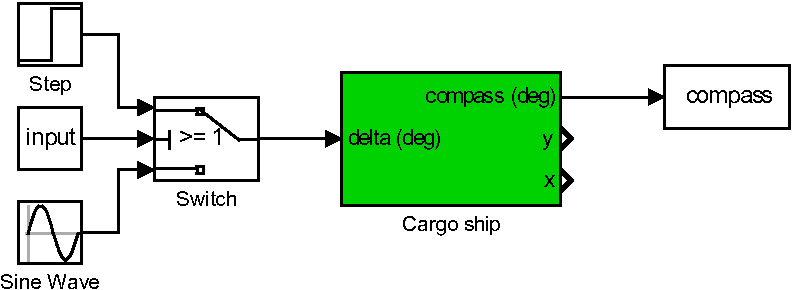
\includegraphics[width=\textwidth]{images/simulink/ship_p1.pdf}
	\label{fig:ship_p1}
\end{figure}






\subsection{Part 5.3}
\begin{figure}[h!]
\caption{Model for Part 5.3 - Top Level - PD Controller takes a setpoint and compass measurement feedback as inputs and returns a rudder input as an output.}
	\centering
		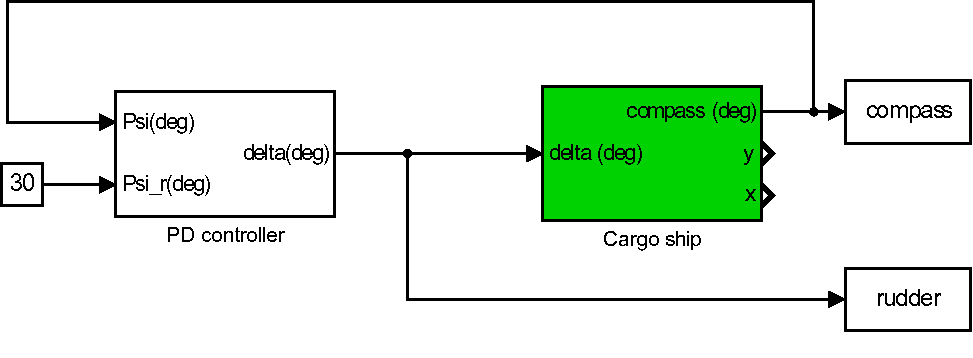
\includegraphics[width=\textwidth]{images/simulink/ship_p3.pdf}
	\label{fig:ship_p3}
\end{figure}


\begin{figure}[h!]
\caption{Model for Part 5.3 - PD Controller - Calculates error, Converts to Radians, Multiplies by Gain, Send through Transfer Function, Converts back to Degrees and clamps the output}
	\centering
		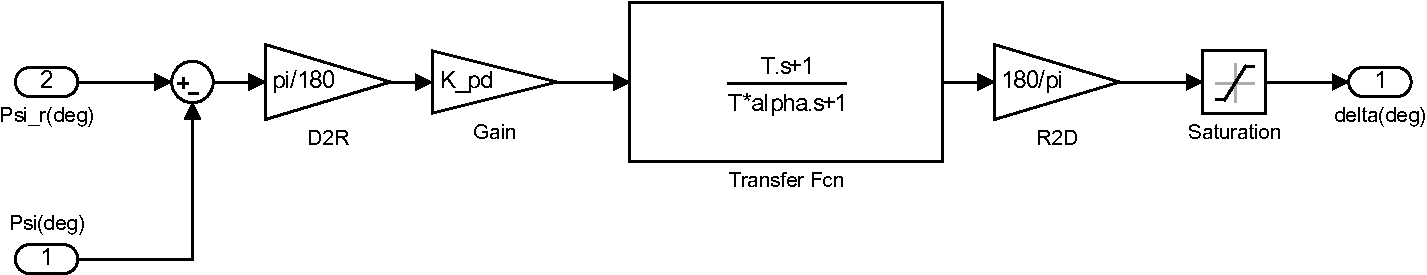
\includegraphics[width=\textwidth]{images/simulink/ship_p3_pd_controller.pdf}
	\label{fig:ship_p3_pd_controller}
\end{figure}







\subsection{Part 5.5}
\begin{figure}[h!]
\caption{Model for Part 5.5 - Top Level - }
	\centering
		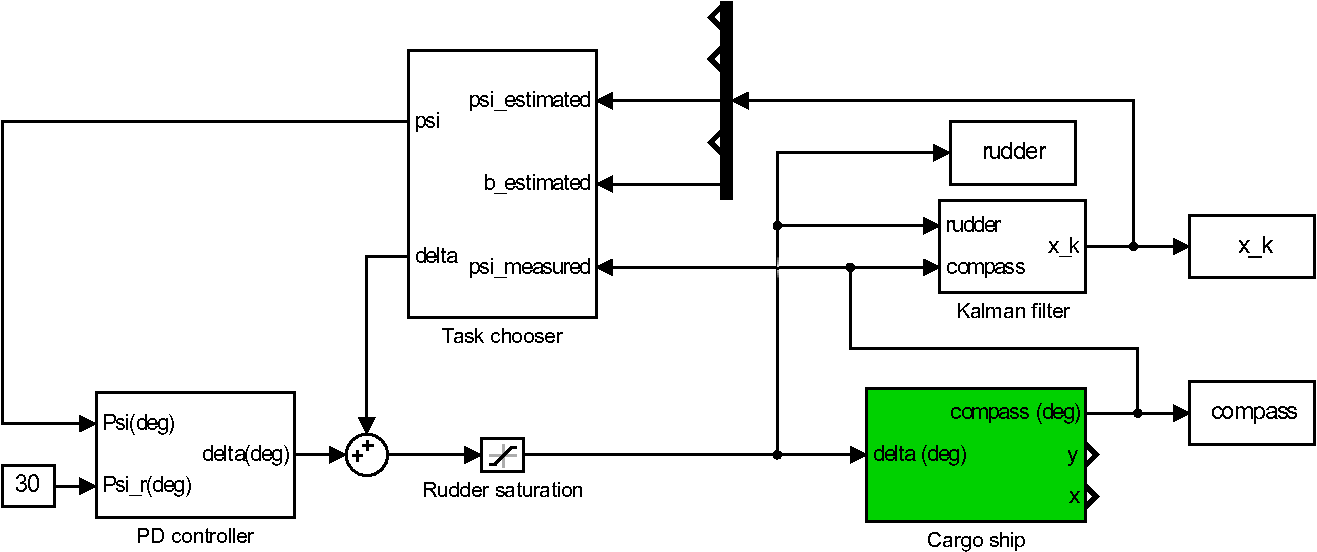
\includegraphics[width=\textwidth]{images/simulink/ship_p5.pdf}
	\label{fig:ship_p5}
\end{figure}

\begin{figure}[h!]
\caption{Model for Part 5.5 - Kalman Filter - }
	\centering
		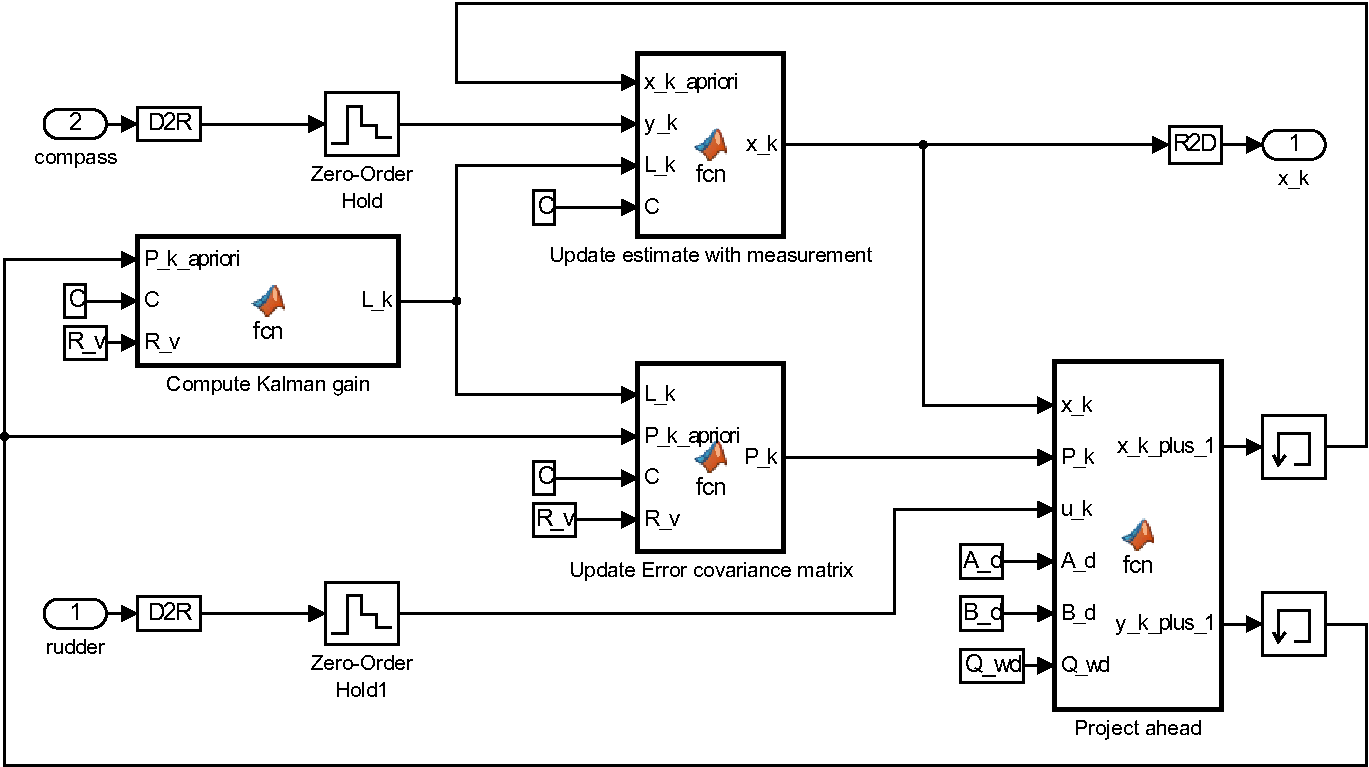
\includegraphics[width=\textwidth]{images/simulink/ship_p5_kalman_filter.pdf}
	\label{fig:ship_p5_kalman_filter}
\end{figure}

\begin{figure}[h!]
\caption{Model for Part 5.5 - Task Chooser - Tunable parameters set in MATLAB for deciding which part of the assignment to simulate. }
	\centering
		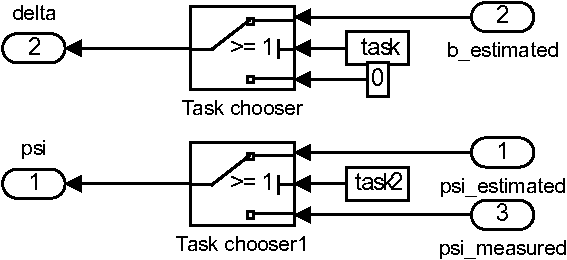
\includegraphics[width=\textwidth]{images/simulink/ship_p5_task_chooser.pdf}
	\label{fig:ship_p5_task_chooser}
\end{figure}


\begin{figure}[h!]
\caption{Model for Part 5.5 - Part B - Basic Model run with input of 0 and only measurement noise. Compass output used to determine variance of the measurement noise.}
	\centering
		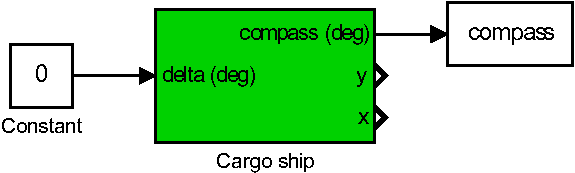
\includegraphics[width=\textwidth]{images/simulink/ship_p5b.pdf}
	\label{fig:ship_p5b}
\end{figure}



\end{subappendices}
